\documentclass[a4paper,10pt]{article}
\usepackage[utf8]{inputenc}
\usepackage{geometry} %自定义布局
\usepackage{multicol} %双栏
\usepackage{graphicx} %图像
\usepackage{amsmath} % 数学单位等等
\usepackage[runin]{abstract} %摘要修改 摘要标题添加到摘要正文段前
\usepackage{booktabs}%三线格
\usepackage{float}%浮点
\usepackage{cite}%引用
\usepackage{pdfpages}%pdf合并
\usepackage{caption}
\usepackage{graphicx, subfig}
\usepackage[colorlinks,
            linkcolor=blue,       %%修改此处为你想要的颜色
            anchorcolor=blue,  %%修改此处为你想要的颜色
            citecolor=blue,        %%修改此处为你想要的颜色,例如修改blue为red
            ]{hyperref}
\usepackage{appendix}
\geometry{a4paper,left=1.6cm,right=1.6cm,top=2cm,bottom=2cm}
\graphicspath{{picture/},{pics/}}
%opening
\title{Enzyme kinetics study of alkaline phosphatase regarding variable reaction time, substrate concentration and enzyme concentration through the colorimetric measurement of deprotonated 4-nitrophenol}
%%%标题加粗
\author{Kangyao Ma }
\date{}


\begin{document}


\maketitle


\setlength{\absleftindent}{0pt}
\setlength{\absrightindent}{0pt}
\setlength{\abstitleskip}{-1.5em}
\abslabeldelim{:}
\renewcommand{\abstractnamefont}{\itshape\bfseries}
\renewcommand{\absnamepos}{flushleft}


\begin{abstract}
\textit{\small The study of influential factors regarding the enzymatic reaction rate is called enzyme kinetics, and it is important to the understanding of enzyme-catalysed reactions. In this research, enzyme kinetics affected by reaction time, substrate concentration and enzyme concentration were studied through three individual experiments using the enzyme alkaline phosphatase and its substrate 4-nitrophenol phosphate, with each experiment having one of the factors above as the only variable. Alkaline sodium phosphate was used to stop the reactions, and tris-hydroxymethyl aminomethane buffer was used to prepare all solutions. The absorbance of the products at 410 nm was measured for analysis. The results suggested that the enzymatic reaction rate decreases over time due to substrate consumption, while the substrate concentration and enzyme concentration were proportional to the rate when their complementary partner was in saturation. }
\end{abstract}


\hrule


\begin{multicols}{2}
\section{Introduction}


%\noindent %无缩进
Enzyme kinetics is the study of the rate of enzyme-catalysed reactions and their affecting factors \cite{robinson2015enzymes}, and the study of enzyme kinetics is essential for the understanding of the mechanism of any enzyme catalysis, as well as the catalytic ability of a specific enzyme under different conditions.

Alkaline phosphatase (AP) is a biological hydrolytic enzyme that plays crucial roles in intracellular biochemical processes like phosphate transportation and metabolism, by catalysing the hydrolysis of phosphate monoesters under alkaline condition \cite{nguyen2017biochemical}\cite{gao2022extraction}\cite{lu2022fluorescent}. 4-nitrophenyl phosphate is a commonly used AP substrate. It will be hydrolysed to 4-nitrophenol and phosphate, and the deprotonated 4-nitrophenol will give a yellow colour with an absorption peak around 405 nm, making the colorimetric results can be related with the enzyme activity \cite{c2000demonstration}\cite{tang2019assays}.

A commonly used method for reactions involving colour-changing products is to measure its absorbance (or optical density, OD) at a certain wavelength, and plot an absorbance curve against reaction time. The relationship between the OD of a molecule and its concentration is expressed by the Beer-Lambert law: $ A=\varepsilon c l $ , where A stands for the absorbance, $\varepsilon$ is the extinction coefficient (M-1cm-1) of that molecule, c is the concentration (M, or mol/L) of that molecule, and l means the path length (cm) of the light, which in case of using an ultraviolet-visible spectrometer is the width of the cuvette \cite{punekar2018enzymes}. Once knowing the A, $\varepsilon$ and l, the rate of the reaction, i.e. the rate of product formation, can be calculated by: $\frac {c} {t} =\frac {A}{\varepsilon l t} (M/min) $ , where t stands for the reaction time in minutes.

The study of enzyme kinetics by measuring the initial velocity (also known as the Michaelis–Menten kinetics) is important as it is in the period with the most prominent inhibitor effects and with least complications \cite{lloyd2021steady}. The two important constants Vmax and Km in the Michaelis–Menten kinetics study can be acquired through a double reciprocal plot of initial velocity against substrate concentration, i.e. the Lineweaver-Burk plot, where the Vmax will be the y-axis intersection and Km being the x-axis intersection \cite{prinz2011enzyme}.

In this research, we have designed three experiments to measure the change in enzyme kinetics with the change in reaction time, substrate concentration and enzyme concentration, aiming to reveal the correlation between these factors and enzyme kinetics.

\section{Material and Method}



\begin{center}
%{\footnotesize Table 1. Materials needed for this experiment}
{Table 1. Materials needed for this experiment}
\begin{table}[H]
%\footnotesize
\begin{tabular}{ll}
\toprule [1pt]
\textbf{Materials}&\textbf{ Explanation  }\\
\hline
Substrate&1 mM 4-nitrophenol phosphate\\
Buffer&0.1 M Tris\\
enzyme&100 \textmu g/mL  alkaline phosphatase\\
stopping-solutions& 0.1 M sodium phosphate \\
\bottomrule [1.5pt]
\end{tabular}
\end{table}
\end{center}

For all three experiments, the buffer used was 0.1 M tris-hydroxymethyl aminomethane buffer (or the Tris buffer), the enzyme used was AP with a concentration of 100 \textmu g/ml in 0.1 M Tris buffer, the substrate was 1 mM 4-nitrophenol phosphate in 0.1 M Tris buffer, and the stop solution was 0.1 M sodium phosphate in 0.1 M Tris buffer. The enzyme, substrate and stopping buffer were stored on ice, and the buffer was kept at room temperature. The enzyme, substrate, and buffer were at pH 9.0, whereas the stopping solution was at pH 11.0. The mixture of substrate and buffer was firstly incubated to allow their temperature to reach the desired degree, before the addition of enzyme. The spectrometer used was with a cuvette width of 1 cm.

\subsection{Changing reaction time}
This experiment aimed to find out the trend of the reaction rate of the enzyme, so that the reaction time of the following reactions can be fixed to fall within the linearly increasing initial velocity range of the enzyme. 15 identical samples in 15 separately labelled test tubes, each composed of 600 \textmu l of substrate, 350 \textmu l of buffer and 50 \textmu l of enzyme, were incubated in a 37 \textcelsius\ water bath to allow the reaction to occur. 2 ml of stopping solution was added to each test tube in a 1-minute interval after the reaction started for 1 minute. The $OD_{410}$ of each sample was measured and recorded for further analysis.

\subsection{Changing substrate concentration}
This experiment aimed to reveal the change in reaction rate with substrate concentration. 8 labelled test tubes were each added with 100 \textmu l – 800 \textmu l of the substrate (in a 100 \textmu l interval) and 850 \textmu l – 150 \textmu l of buffer (in a 100 \textmu l interval) respectively, as well as 50 \textmu l of the enzyme to make up a total 1 ml solution. All samples were incubated in the 37 \textcelsius\ water bath for 1 minute to allow the reaction to take place, then 2 ml of stopping solution was added to each sample simultaneously to ensure they had the same reaction time. The OD410 of each sample was measured and recorded for further analysis.


\subsection{Changing enzyme concentration}

This experiment aimed to discover the change in reaction rate with enzyme concentration. 11 labelled test tubes were added with 800 \textmu l of substrate, and 200 \textmu l – 150 \textmu l of buffer (in a 5 \textmu l interval) respectively. 0 \textmu l - 50 \textmu l (in a 5 \textmu l interval) of the enzyme were then added to each tube to make up a total 1 ml solution. After reacting in the 37 \textcelsius\ water bath for 1 minute, 2 ml of stopping solution was added to each sample simultaneously to ensure they had the same reaction time. The $OD_{410}$ of each sample was measured and recorded for further analysis.


\iffalse
\begin{center}
{\footnotesize Table 2. Outline of the mutagenesis for each plate}
\vspace{0pt}
\begin{table}[H]
\footnotesize
\begin{tabular}{ccccc}
\toprule [1.5pt]
Plate Number&Cell dilution to be plated&Plate type&Tryptophan concentration(\textmu g/mL)&Treatment\\
\hline
1&$10^0$&SA3&0&$Trp^+$ strain and $Trp^-$ strain\\
2&$10^0$&SA3&0&None\\
3&$10^0$&SA2&1&None\\
4&$10^0$&SA1&0.25&None\\
5&$10^{-5}$&NA&Non-limiting&None\\
6&$10^{-6}$&NA&Non-limiting&None\\
7&$10^0$&SA2&1&Spot test with 1\% MMS\\
8&$10^0$&SA2&1&Spot test with 1\% MMS\\
9&$10^0$&SA2&1&Spot test control (water)\\
10&$10^0$&SA1&0.25&Treat with 1\% MMS then plate\\
11&$10^0$&SA2&1&Irradiate with UV light for 20 sec\\
12&$10^0$&SA2&1&Irradiate with UV light for 40 sec\\
\bottomrule [1.5pt]
\end{tabular}
\end{table}
\end{center}
\fi


%\begin{figure}[htbp]
%\centering
%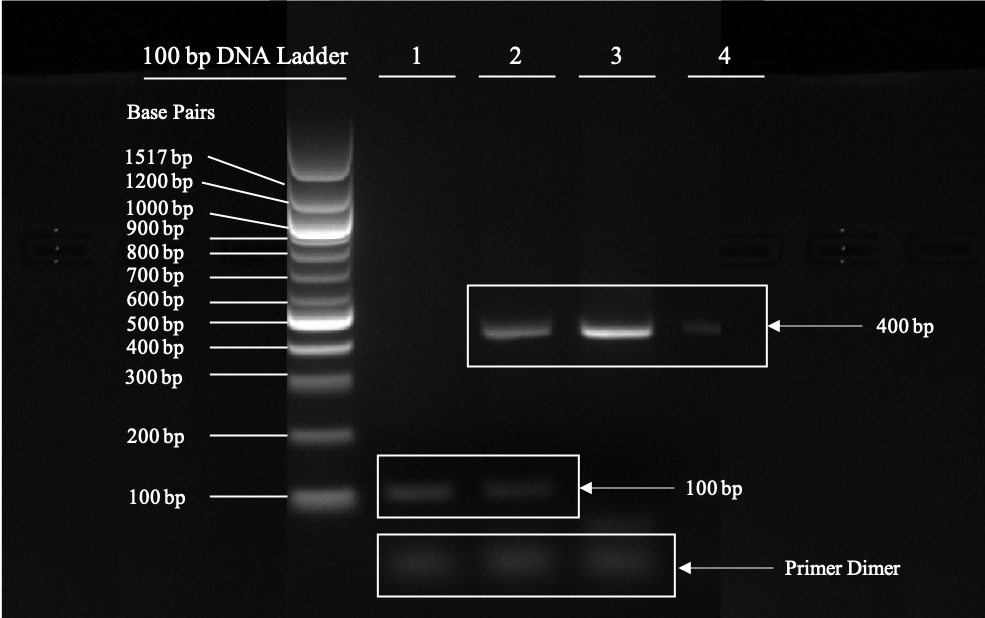
\includegraphics{tpa25.png}
%\caption{bionux}
%\end{figure}


\section{Results and Analysis}


\subsection{Time Course Assay for Subsequent Reaction Time and Initial Velocity}
Before examining the effects of various parameters, an initial velocity was estimated using an enzyme concentration of 0.005 mg/mL and a substrate concentration of 0.6 mM. At the beginning of the reaction, rates are proportional to the concentrations of enzyme-substrate complexes. Controlling time is crucial, so we aimed to find and set reasonable reaction periods where product formation increases linearly over time to prevent substrate depletion. According to the Beer-Lambert law, absorbance was converted to product concentration, and a plot of reaction rates was generated (Figure 1A). The data indicate that the first six minutes show a linear product increase, with rates declining after ten minutes. Substrate depletion contributes to these rate reductions. Figure 1B shows a curve-fitting result using only the first five minutes of data, with an R² of 0.998, further supporting the linear rate range. Overall, with an enzyme concentration of 0.005 mg/mL, a reaction period within the first five minutes is suitable for subsequent experiments due to its consistent linear product increase.

\iffalse
\begin{figure}[H]
\centering
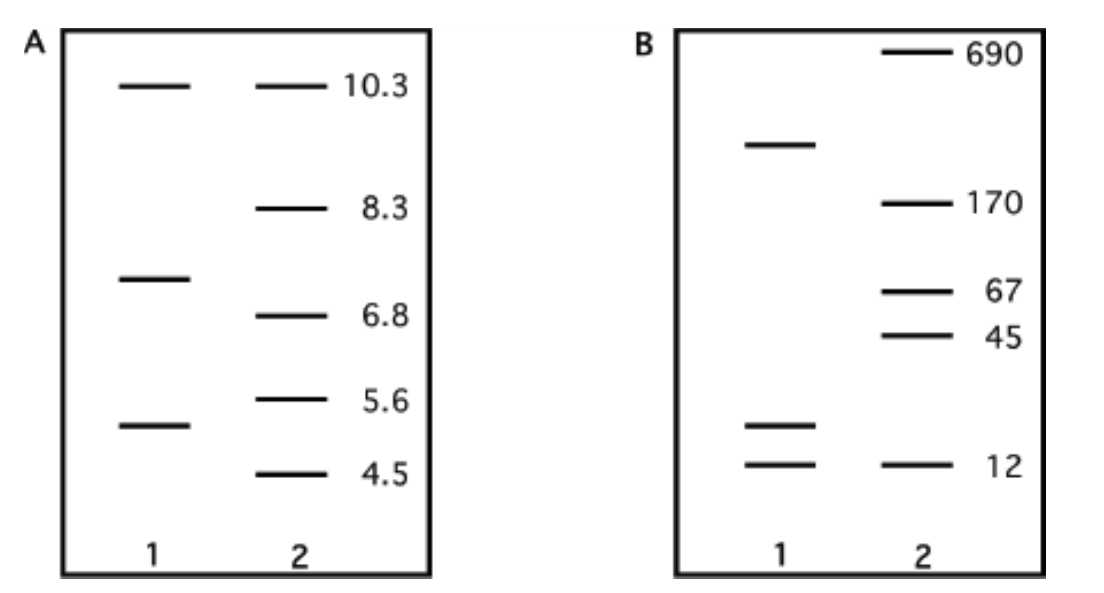
\includegraphics[width=0.45\textwidth]{sds.png}
\captionsetup{font={scriptsize,bf,stretch=1}}
\caption{\scriptsize \textbf{Electrophoretic Analyses Results of Protein Mixture. The picture on the left is isoelectric focusing of a protein sample. The three protein bands are represented by 1, 2, and 3. The picture on the right is the polyacrylamide gel electrophoresis result of the protein sample. The three protein bands are represented by a, b, and c. }}
\label{fig1}
\end{figure}


\begin{center}
{Table 2. Count of bacterial colonies on each plate}
\vspace{0pt}
\begin{table}[H]
\setlength{\tabcolsep}{5pt}

\begin{tabular}{llll}
\toprule [1pt]
Component&pI value & Component & MW\\
\hline
protein 1 & 10.3 & protein a & 298\\
protein 2 & 7.5 & protein b & 19\\
protein 3 & 5.3 & protein c & 12\\
\bottomrule [1pt]
\end{tabular}
\end{table}
\end{center}
\fi


\begin{figure}[H]
\centering
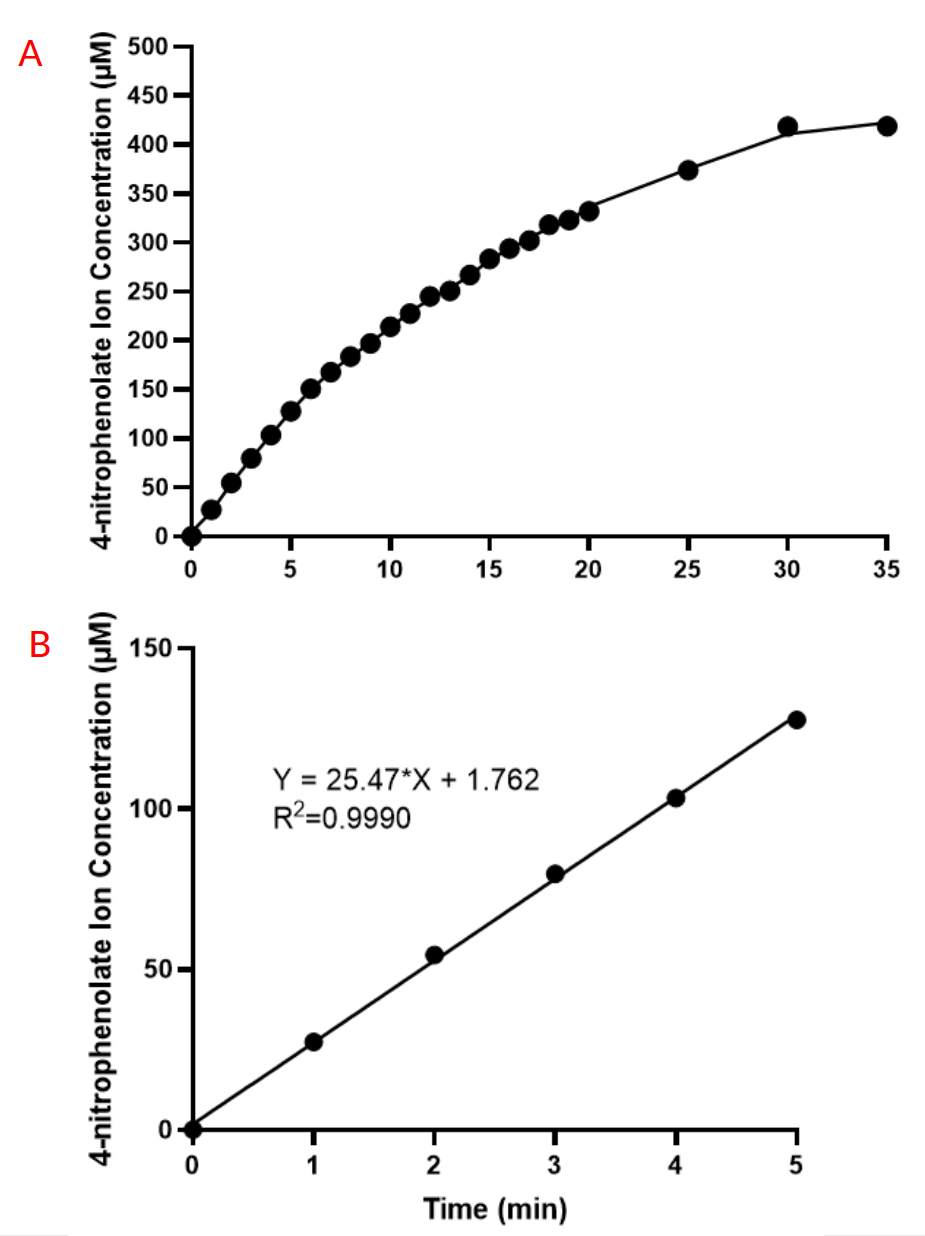
\includegraphics[width=0.45\textwidth]{fig1.png}
\captionsetup{font={scriptsize,bf,stretch=1}}
\caption{\scriptsize \textbf{(A)Time course assay results for AP. (B) Curve fitting is built from separated data of the first five minutes.}}
\label{fig2}
\end{figure}


Since Vmax and Km are not determined in this assay, calculating initial velocities (V0) via the Michaelis-Menten equation is not feasible. Therefore, V0 is estimated only at the reaction's initiation. Although the first five minutes generally fall within linear ranges, instantaneous rates decrease over time. Thus, the first minute's data is used for V0 estimation, with instantaneous and average velocities within this period being 27.26 \textmu M/min and 27.37 \textmu M/min, respectively. Ideally, rates at the very beginning are closer to actual initial velocities, though even the first minute might be too long, leading to biased V0 approximations. Both estimates are similar; however, instantaneous rates reflect speeds at the start of the first minute, while the average rate represents the mean velocity within that minute, meaning neither exactly corresponds to the theoretical V0.





\subsection{Substrate Concentration Assay}


After characterizing possible linear reaction ranges, we examined the impact of substrate concentrations. The time course assay, with 0.6 mM substrate and 0.005 mg/mL enzyme, showed that products increase linearly for at least five minutes with sufficient substrates. The reaction period should be long enough to reach steady-state conditions and distinguish velocities between sufficient and inadequate substrates. Thus, reaction periods and enzyme concentrations were unified as five minutes and 0.005 mg/mL, respectively, for each substrate concentration group. Figure 2A illustrates the effect of substrate doses on reaction rates, reflecting a process where velocities gradually approach Vmax as substrate concentration increases and Km becomes less significant. At high substrate concentrations, enzymes are saturated, and reaction rates are limited by Vmax. Before 0.3 mM, rates increase dramatically with substrate doses. Although velocities increase more slowly with higher substrate concentrations, they continue to rise gently until 0.9 mM without reaching a plateau.


\begin{figure}[H]
\centering
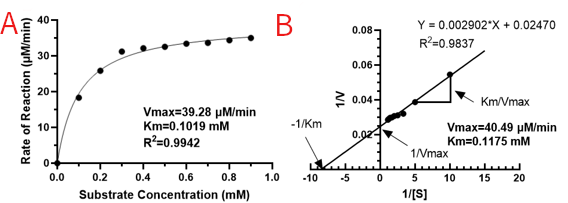
\includegraphics[width=0.45\textwidth]{fig21.png}
\captionsetup{font={scriptsize,bf,stretch=1}}
\caption{\scriptsize \textbf{(A) Effects of substrate concentration on reaction rates. Intervals for substrate concentration are 0.1 mM from 0 to 0.9 mM. (B) Lineweaver-Burk plot. This is made using double reciprocal methods of velocities and substrate concentrations with extensions to intersect with X-axis.}}
\label{fig3}
\end{figure}


Using the substrate-rate correlation, a non-linear regression fitting curve based on the Michaelis-Menten model was generated (Figure 2A). The Vmax and Km obtained from this curve are 39.28 \textmu M/min and 0.1019 mM, respectively. Additionally, a Lineweaver-Burk plot (Figure 2B) was constructed to traditionally determine Vmax and Km, which were found to be 40.49 \textmu M/min and 0.1175 mM, respectively. These values are generally consistent with the Michaelis-Menten model, with differences potentially due to the lack of constant maximum velocities. The Vmax values suggest that the slow increase in reaction rates up to 0.9 mM substrate may be because the highest substrate concentration does not fully reach Vmax. The velocity at 0.9 mM substrate is about 35 \textmu M/min, slightly less than the estimated Vmax of around 40 \textmu M/min. With these Vmax values, the AP-specific activity can be estimated at 7.856 and 8.098 $\mu mol\cdot mg^{-1}\cdot min^{-1}$ , indicating the enzyme's turnover capacity. At a substrate concentration of 0.6 mM, the initial velocity from the Michaelis-Menten equation is about 33.5 \textmu M/min, differing from the estimated V0 of about 27 \textmu M/min in the time course assay, which was only a rough approximation.



\subsection{Enzyme Concentration Assay}
Although enzyme amounts are usually small in enzymatic reactions, they can significantly influence enzyme kinetics and reaction rates. Additional experiments were conducted to examine the effects of enzyme concentration. In previous experiments with an enzyme concentration of 0.005 mg/mL and a substrate concentration of 0.6 mM over five minutes, substrate depletion was not an issue, but the substrate concentration was insufficient to reach Vmax. Therefore, a substrate concentration of 0.8 mM and gradually decreasing enzyme doses were used to avoid substrate insufficiency. Results are presented in Figure 3. The data indicate that reaction rates increase linearly with enzyme concentration, meaning that when substrates are sufficient, nearly all enzyme molecules are bound to substrates, forming enzyme-substrate complexes. Reaction rates may not increase further because there are limited free enzyme molecules available to bind to additional substrate molecules. Thus, reaction rates approach maximum velocities under the corresponding enzyme concentrations and are limited by the turnover rate of AP, determined by AP's catalytic efficiency. The overall specific enzyme activity of AP, implied by the slope of the line, is estimated in this session as 7.917 $\mu mol\cdot mg^{-1}\cdot min^{-1}$, consistent with previous estimations of 7.856 and 8.098 $\mu mol\cdot mg^{-1}\cdot min^{-1}$. At an enzyme concentration of 0.005 mg/mL, the reaction rate is 40.45 \textmu M/min, close to the estimated Vmax but showing some discrepancy with results from the substrate concentration assay. This difference may be due to absorbance inconsistencies from variations in the blanks used for OD value measurements.

\begin{figure}[H]
\centering
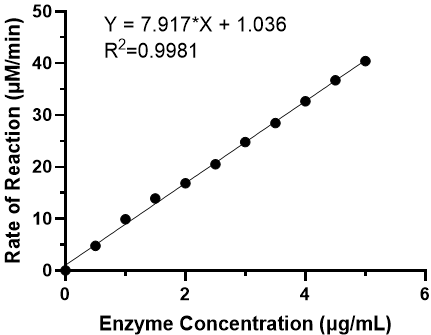
\includegraphics[width=0.4\textwidth]{fig3.png}
\captionsetup{font={scriptsize,bf,stretch=1}}
\caption{\scriptsize \textbf{Effect of changes in enzyme concentration on reaction rate.}}
\label{fig5}
\end{figure}


\iffalse
\begin{figure*}
\centering
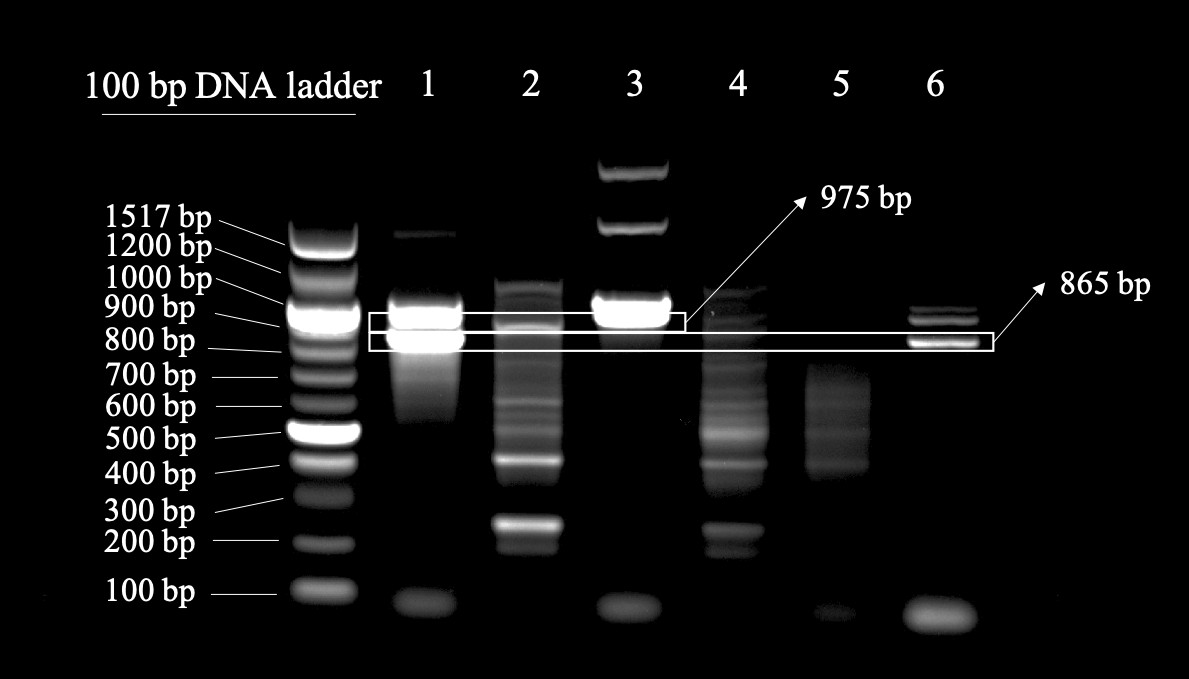
\includegraphics[width=0.95\textwidth]{gel.jpg}
\captionsetup{font={scriptsize,bf,stretch=1}}
\caption{\scriptsize \textbf{PCR verification for putative transformants 1 and 2. Lanes 1 and 2 were set as negative controls which added the genome of the negative strain as a template. Lanes 3 and 4 added the genome of transformant 1 as a template. Lanes 5 and 6 added the genome of transformant 2 as a template. Samples of lanes 1, 3 and 5 were amplified DNA with diagnostic primers ANID\_08549F and ANID\_08549R. Samples of lanes 2, 4 and 6 were amplified DNA with diagnostic primers ANID\_08549F and Af-Revers.}}
\label{fig3}
\end{figure*}


\begin{center}
{Table 3. The Concentration of Protein Samples Through the Bradford Method.}
\vspace{0pt}
\begin{table}[H]
\setlength{\tabcolsep}{5pt}
\begin{tabular}{lc}
\toprule [1pt]
Components&Concentration(mg/mL)\\
\hline
Original Mixture & 5.2\\
IEX unbound & 1.7 \\
IEX bound & 4.3 \\
GFC peak 1 & 1.9 \\
GFC peak 2 & 2.0\\
\bottomrule [1pt]
\end{tabular}
\end{table}
\end{center}


\begin{center}
{Table 4. Data related to three proteins}
\vspace{0pt}
\begin{table}[H]
\setlength{\tabcolsep}{5pt}
\footnotesize
\begin{tabular}{llll}
\toprule [1pt]
Proteins&MW (kDa)& pI & Protein Fraction\\
\hline
Cytochrome c & 11.83 & 9.59 & IEX unbound\\
Myoglobin & 17.08 & 7.20 & GFC peak 2\\
Ferritin-light chain & 19.98 & 5.37 & GFC peak 1\\
Ferritin-heavy chain & 21.27 & 5.41 & GFC peak 1\\
\bottomrule [1pt]
\end{tabular}
\end{table}
\end{center}



\begin{center}
{Table 5. The Molecular Weight of Each Protein from SDS-PAGE and Bioinformatics Search.}
\vspace{0pt}
\begin{table}[H]
\setlength{\tabcolsep}{5pt}
\footnotesize
\begin{tabular}{llll}
\toprule [1pt]
Proteins&MW (database)&MW (SDS-PAGE)\\
\hline
Cytochrome c & 11.83 & 15.85\\
Myoglobin & 17.08 & 20.14\\
Ferritin-light chain & 19.98 & 23.61\\
Ferritin-heavy chain & 21.27 & 26.36\\
\bottomrule [1pt]
\end{tabular}
\end{table}
\end{center}
\fi



\section{Discussion and Conclusion}
According to the analysis of the results, it was observed that the enzyme reaction rate decreases over time. This decrease in the reaction rate can be attributed to a reduction in substrate concentration due to the ongoing reaction. The experimental data also revealed that at low substrate concentrations, enzyme-substrate complexes were not formed adequately, resulting in lower reaction rates despite different Vmax values at varying concentrations. By employing a Lineweaver-Burk plot, a linear relationship was established and allowed for determination of Km and Vmax under these conditions. In investigating the impact of enzyme concentration on rate of reaction, under conditions that varied the enzyme concentration and ensured adequate substrate, the reaction rate was found to be proportional to the enzyme concentration.

In this study, spectrophotometric determination of product concentration was employed as an indicator of reaction rate while controlling other variables. Stable reagents were utilized without any requirement for complex pre-treatment or preparation procedures such as advanced biochemistry or quantum dot/polymer synthesis. Furthermore, by initially examining time and concentration variables and plotting corresponding graphs, it ensured that when altering enzyme concentration, the reaction rate corresponded to Vmax values thus ensuring reliable data for enzyme concentration studies. One limitation of this study is related to difficulties encountered during agitation steps under water bath conditions which necessitated brief shaking intervals for separating substrates from water baths; this may have influenced results slightly. Additionally, since only alkaline phosphatase was investigated in this study, generalizability of findings across all enzyme proteins cannot be determined; further research involving different enzymes is warranted.

The study primarily investigated the reaction rate of alkaline phosphatase under varying conditions in order to determine the optimal enzyme concentration and other parameters for further research. Under the condition of sufficient substrate, the enzyme molecules almost all form complexes with the substrate, which is related to the structure of the enzyme protein itself. Alkaline phosphatases are a group of isoenzymes, and each monomer has an active site, and one site can only bind to one molecule of substrate at the same time. Therefore, under the condition of sufficient substrate concentration, the reaction rate will increase linearly with the increase of enzyme concentration. Although higher enzyme concentration changes the reaction rate, the enzyme activity is not altered, and the effect of temperature on alkaline phosphatase activity is critical. At low temperatures, both enzyme and substrate molecule movements are hindered, resulting in decreased reaction rates and enzyme activity\cite{dede2002effect}. Conversely, high temperatures disrupt weak molecular forces like hydrogen bonding and ionic bonding within the enzyme's structure, leading to spatial structure destruction. The three-dimensional configuration of the enzyme is essential for its functionality; hence, high temperatures cause a decline in enzyme activity\cite{bzura2018photometric}. Moreover, experiments on enzyme activity can also manipulate other factors such as metal ions by altering the molecular structure of the enzyme to influence its overall performance. Different metal ions may exert diverse effects on alkaline phosphatase activity. In Jennifer's study, it was discovered that magnesium and zinc positively impact alkaline phosphatase by enhancing its enzymatic function. Specifically, alkaline phosphatase consists of a dimer containing two zinc atoms and one magnesium atom per monomer with inorganic phosphate bound between each active site's two zinc atoms\cite{murphy1995mutations}. On the contrary, heavy metal ions like Hg2+ and Pb2+ inhibit enzymatic activity either through occupying the active center or binding to sulfhydryl groups, amine groups or carboxyl groups within the enzyme molecules. Therefore, investigating various metal ions' effects on enzymatic activities can be conducted as part of this study.

In this study, research investigated the variation in the reaction rate of alkaline phosphatase under three different conditions (time, substrate concentration, and enzyme concentration) by controlling variables. Research ensured that the enzyme concentration was changed while maintaining a constant Vmax rate, and the linear relationship was obtained by measuring the reaction rate. The results of our study also revealed time-rate curves and substrate concentration-rate curves, providing evidence for their linear relationship. Additionally, research observed that temperature influences enzyme activity; both high and low temperatures lead to a decrease in enzyme activity. Moving forward, the next step is to explore the reaction rate of different types of enzymesto confirm the reliability of the research conclusions, and by changing the temperature condition and adding different metal ions by changing the influence of the enzyme activity for the reaction rate.


\bibliographystyle{unsrt}
\bibliography{reference}

\end{multicols}


\clearpage

\iffalse
\begin{appendices}
\section*{Appendix A. Data Analysis Sheet}\label{secA}

\textbf{Authors:} Mingbai.Zeng, Kangyao.Ma, Haozhan.Yuan, Yimeng.Yuan\\
\textbf{Date:} 2024.4.12\\
\textbf{Gene Name:} Uncharacterized\\
\textbf{Systemic Name:} AN8549, ANID\_08549\\
\textbf{Description:} Uncharacterized protein\\
\textbf{References:}For A. nidulans – none available\\
\textbf{GO annotation:}\\
GO:0008150 Biological Process\\
GO:0005575 Cellular Component\\
GO:0003674 Molecular Function\\
\textbf{S. cerevisiae Homologue:}\\
\textbf{Protein Sequence:}\\
\textgreater AN8549-T $\mid$ Aspergillus nidulans FGSC A4 $\mid$ segment length=394\\
\texttt{MPVDNYGVLKCRAITYKLEDGQQSPRAPQLSLYVRDTGSPTSQLNGHLQEARAGLPVHRAAINITSGDLDDSR\\
LAYWVNHQIGQNPIVNRLSQLEYGFHPVENNKTLGLDYIRDSLFTSTNGRLLPHDIPGQYTDIIDVLSPYIQH\\
AVREKANLYLFGSESRSDTRGSAPVIHNIHMNQGNARKFRADDGVFQDGGLIFHFPCARPDSDTGCVEDRPRG\\
EWLGIFLAFASQAVHTNPSSGHAISGVGWSDILRPDIIEEGVVIREARLHLDSSGTDADAVTDESETGARPCI\\
GRRKSISLTVTLSNHTNRAVRLGDWTIRNRSGCVHTLPRGIALRPMVDQHFELGDYTLSEDGDTILLLNEHGL\\
KVDGVSYNSAQEGMGLKGKGKGGSIVFVH}\\
\textbf{Pfam domains:}\\
1 Lamin tail domain superfamily, Lamin A/C globular tail domain\\
\textbf{Primers used for Deletion cassette:}\\
5 forward: \texttt{GTAACGCCAGGGTTTTCCCAGTCACGACGGAGACTCATACAGCCCTACC}\\
5 Reverse: \texttt{ATCCACTTAACGTTACTGAAATCTCAAGACCCCGTAGTTGTC}\\
3 forward: \texttt{CTCCTTCAATATCATCTTCTGTCGAGAGAAAAGGAGTGAGGTG}\\
3 Reverse: \texttt{GCGGATAACAATTTCACACAGGAAACAGCAAGCAGACAGTAACCCTAGC}\\
\textbf{Diagnostic primers and expected product size for wild type:}\\
ANID\_08549F: \texttt{TCGCAGGTCCCAGTGATG}\\
ANID\_08549R: \texttt{GTCCATCCCAGCCATTTG}\\
PCR product size in the wild type: 975 bp\\
\textbf{Diagnostic primers and expected product size for mutant:}\\
ANID\_08549F: \texttt{TCGCAGGTCCCAGTGATG}\\
Af-Rev: \texttt{CCACTTAACGTTACTGAAATC}\\
PCR product size in the mutant: 865 bp\\
\textbf{Annotated DNA sequence:}\\
(Note: The sequence in red indicates the intron of the genome, and the sequence in blue indicates the open reading frame (ORF) of the gene ANID\_08549 and PyrG gene. The sequences that are highlighted are the primers used in the lab session)
\begin{figure}[H]
\centering
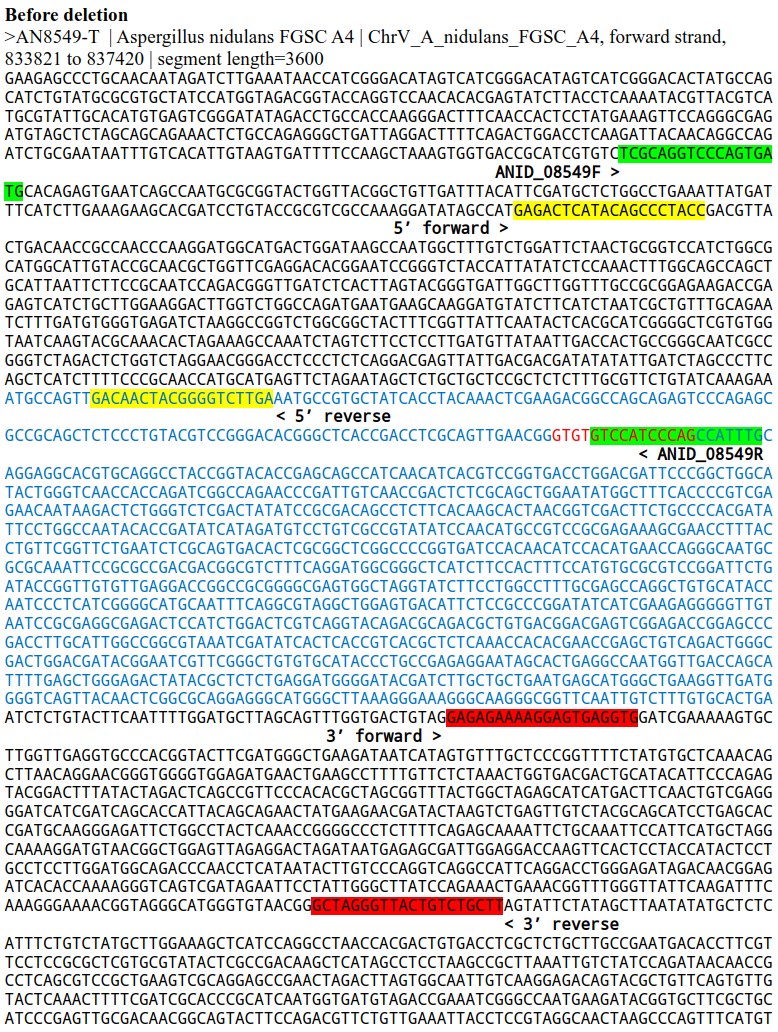
\includegraphics[width=0.95\textwidth]{before.png}
%\captionsetup{font={scriptsize,bf,stretch=1}}
%\caption{\scriptsize \textbf{Amplification of putative transformants and negative strain. Negative strain (A), transformants 1 (B) and transformant 2 (C).}}
%\label{fig4}
\end{figure}

\begin{figure}[H]
\centering
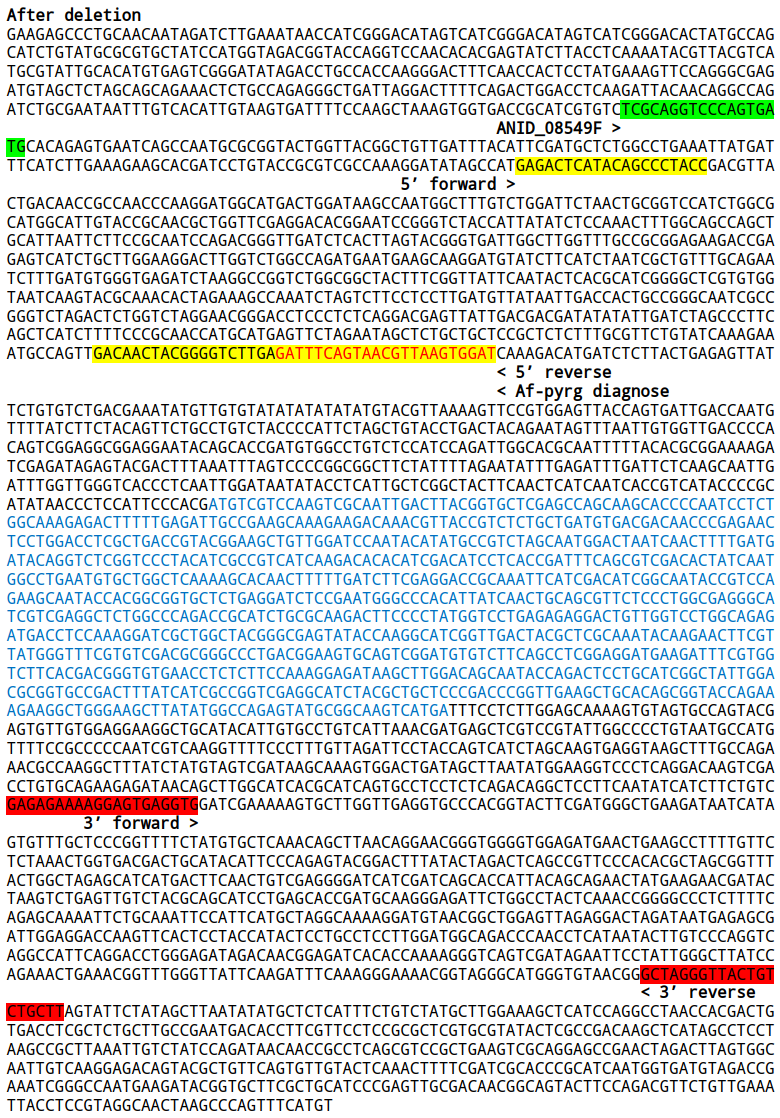
\includegraphics[width=0.95\textwidth]{after.png}
%\captionsetup{font={scriptsize,bf,stretch=1}}
%\caption{\scriptsize \textbf{Amplification of putative transformants and negative strain. Negative strain (A), transformants 1 (B) and transformant 2 (C).}}
%\label{fig4}
\end{figure}


\section*{Appendix B. Prediction of molecular structure of hypothetical protein AN8549}\label{secB}

\begin{figure}[H]
\centering
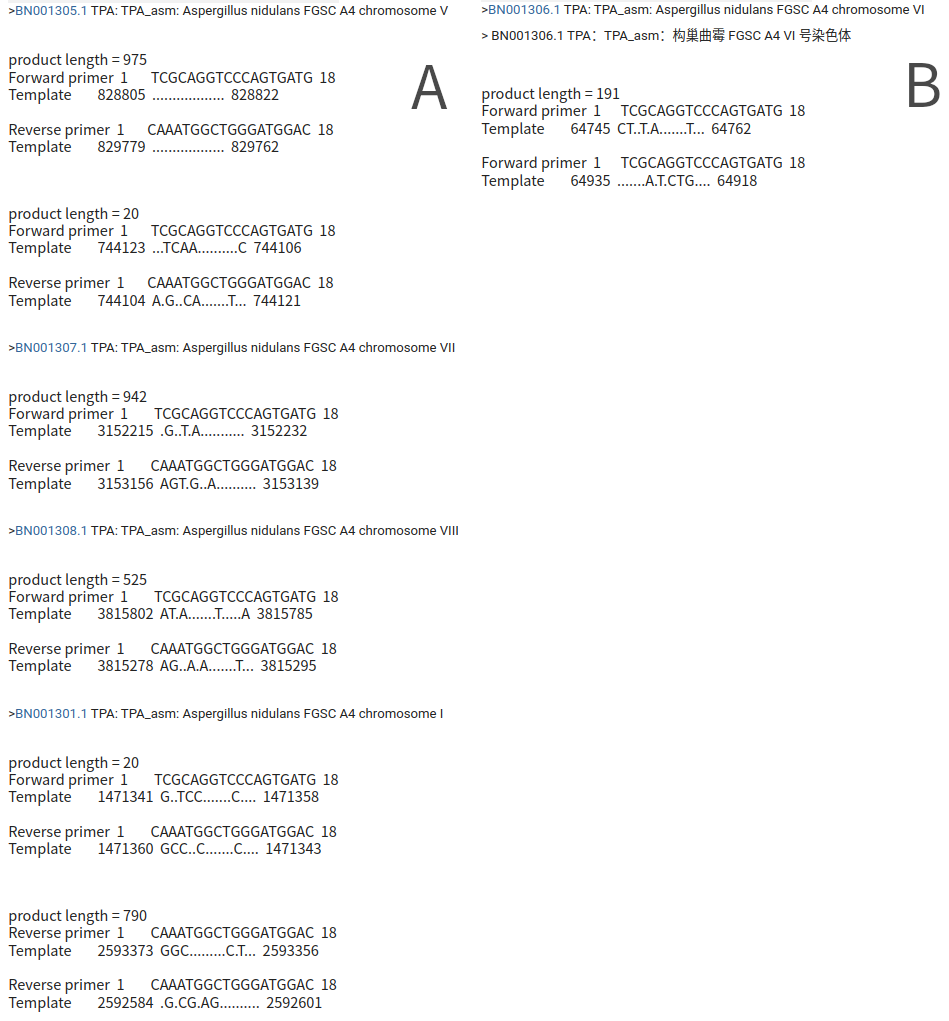
\includegraphics[width=0.95\textwidth]{primerblast.png}
%\captionsetup{font={scriptsize,bf,stretch=1}}
%\caption{\scriptsize \textbf{Amplification of putative transformants and negative strain. Negative strain (A), transformants 1 (B) and transformant 2 (C).}}
%\label{fig9}
\end{figure}


\section*{Appendix D. Prediction of domain structure of hypothetical protein AN8549\cite{paysan2023interpro}}\label{secD}

\begin{figure}[H]
\centering
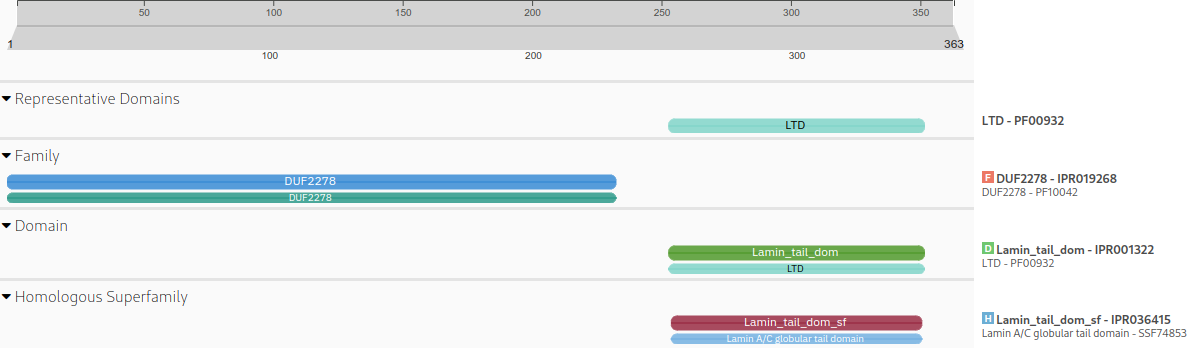
\includegraphics[width=0.95\textwidth]{BO83DRAFT_454721domain.png}
%\captionsetup{font={scriptsize,bf,stretch=1}}
%\caption{\scriptsize \textbf{Amplification of putative transformants and negative strain. Negative strain (A), transformants 1 (B) and transformant 2 (C).}}
%\label{fig5}
\end{figure}

\end{appendices}
\fi


\end{document}
